%%%%%%%%%%%%%%%% Springer %%%%%%%%%%%%%%%%%%%%%%%%%%%%%%%%%%
\documentclass{svproc}

% to typeset URLs, URIs, and DOIs
\usepackage{url}
\def\UrlFont{\rmfamily}

% Graphics, Math, Tables
\usepackage{graphicx}
\graphicspath{{figures/}} %Setting the graphics path
\usepackage{amsmath}
\usepackage{multicol}
\usepackage{array}
\usepackage{multirow}
\usepackage{footmisc}
%\usepackage[numbers,sort,compress]{natbib}
\usepackage[sort&compress,numbers]{natbib}
%\usepackage[numbers]{natbib}
\bibliographystyle{spbasic_unsort}
\usepackage{chngpage}
\usepackage{placeins}


\begin{document}
\mainmatter              % start of a contribution
%
\title{A Bayesian Network Approach to Evaluate Shipboard Launch and Recovery Performance in Early-Stage Ship Design}
%
\titlerunning{Bayesian Networks in Ship Design}  % abbreviated title (for running head)
%                                     also used for the TOC unless
%                                     \toctitle is used
%
\author{James A. Coller\inst{[0000-0003-3825-923X]} \and David J. Singer\inst{[0000-0002-5293-6236]}}
%
\authorrunning{Coller et al.} % abbreviated author list (for running head)
%
%%%% list of authors for the TOC (use if author list has to be modified)
\tocauthor{James A. Coller, David J. Singer}
%
\institute{Department of Naval Architecture and Marine Engineering \\ University of Michigan, Ann Arbor, MI, United States,\\
\email{jcoller@umich.edu},\\ Web Page:
\texttt{https://ancr.engin.umich.edu/}
}

\maketitle              % typeset the title of the contribution

\begin{abstract}
Vessel performance in shipboard launch and recovery operations is a critical element of its overall mission effectiveness. Both commercial and military vessels are required to launch and recover a variety of manned and unmanned platforms including submersibles, small boats, aircraft, and amphibious vehicles. A fundamental attribute of these launch and recovery operations is their dependence on a number of probabilistic factors such as environmental conditions and design factors associated with the vessel and the platforms. To facilitate effective launch and recovery operations, ship designers require a design method that takes into account these probabilistic factors to gain a better understanding the implications of launch and recovery on a variety of early stage design decisions. Recent advancements in design tools and methodologies have pushed critical decisions earlier in the design process which necessitates evaluating mission critical systems sooner as well. \\

This paper presents an application of Bayesian networks for evaluating the performance of shipboard launch and recovery operations. Bayesian networks provide a framework for understanding system interdependencies by modeling and analyzing conditional probabilities between variable pairs. In previous ship design research, Bayesian networks have been applied to risk modeling and the examination of principal particulars. \\

This research utilizes Bayesian networks to model the environmental and design factors that contribute to the performance of launch and recovery operations, using a level of information that is consistent with early-stage ship design. These networks are analyzed and examined to assess the impact of the overall design attributes on those factors. A ship design case study is presented to demonstrate the method and elucidate the driving interdependencies in launch and recovery operations. 

% We would like to encourage you to list your keywords within
% the abstract section using the \keywords{...} command.
\keywords{Bayesian Networks, Ship Design, Launch and Recovery, Design Tools, Unmanned Vehicles, Causal Dependency}
\end{abstract}
\clearpage % because it looks weird otherwise with 2 lines on the first page

%
\section{Introduction}
%
\subsection{Problem and Approach}

Advancements in naval architecture continue to push the boundaries of how much of the design space can be explored for a given ship within time and budgetary constraints. With methodologies that require large portions of the design space to be investigated, such as set based design (SBD), \cite{singer_sbd_09}  the design space needs to be explored in a computationally efficient manner while providing novel information that enables decision making with limited information. 

Early stage design requires efficient design tools to effectively examine a given design and evaluate the design performance \cite{whitcomb_naval_1998}. These tools are used to evaluate the potential ship designs and ensure that the key design requirements are met. While these tools have inherent biases and will have an impact on the decision making process \cite{sypniewski_framework_2017}, they remain necessary in modern ship design. 

Naval ships are often tasked with the launch and recovery of additional systems, both manned and unmanned, including boats, helicopters, unmanned underwater vehicles (UUVs), unmanned aerial vehicles (UAVs), and unmanned surface vehicles (USVs). The design of the ship can have a large impact on the effectiveness of these operations, in addition to environmental conditions and operating procedures. Design features such as well decks, stern ramps, davits, cranes, and helicopter pads can be complicated to integrate and evaluate. 

As the use of unmanned vehicles increases, these operations will continue to increase in complexity. The US Navy has stated it plans to continue rolling out unmanned vehicles to integrate with the fleet, across the skies \cite{crs_drones}, the surface \cite{lagrone_navy_2019}, and subsea \cite{us_navy_navy_2004}. Unmanned and autonomous vehicles can be more difficult to launch and recover without human operator guidance and with an increased number of systems that must flawlessly execute. 

This paper investigates a novel approach to this problem by using a Bayesian network to evaluate the environmental and ship design factors for a shipboard launch and recovery system. The Bayesian Network will allow the designer to evaluate the interdependencies of the design decision and evaluate the expected satisfaction with the overall design. The network structure allows the designer to simulate satisfaction for a wide range of vehicles and complex systems. 

In the remainder of the paper, an introduction to launch and recovery systems and Bayesian networks will be presented. The methodology is explained, and a case study is presented to highlight the network structure and examine variable sensitivity. Additional opportunities for further work and implications are discussed. 

\subsection{Launch and Recovery Design Space}

In naval ship design, many mission profiles include launching and recovering any number of other vehicles from the ship platform. A given design may be tasked with having several launch and recovery areas such as well decks, flight decks, and davits \cite{navy_fact_file},\cite{orourke_navy_2018}. Multi-mission ships are tasked with flexible spaces that can serve a wide variety of mission capabilities depending on the call to service and the changing geo-political climate \cite{orourke_coast_2019}, \cite{orourke_lcs_2018}. 

Within this design space, the possible vehicles to be launched or recovered are numerous. Categorically, they include aerial, surface, and subsea vehicles. Within these categories, dozens to thousands of variants exist. Figures~\ref{fig:navy_rhib} and~\ref{fig:navy_lcac} highlight some of the variety a single ship may see. Additional unique missions may include recovering non-propulsive vehicles such as a NASA landing module \cite{nasa_2018}. 

\begin{figure}[hbt]
	\centering
	\begin{minipage}[b]{0.45\textwidth}
		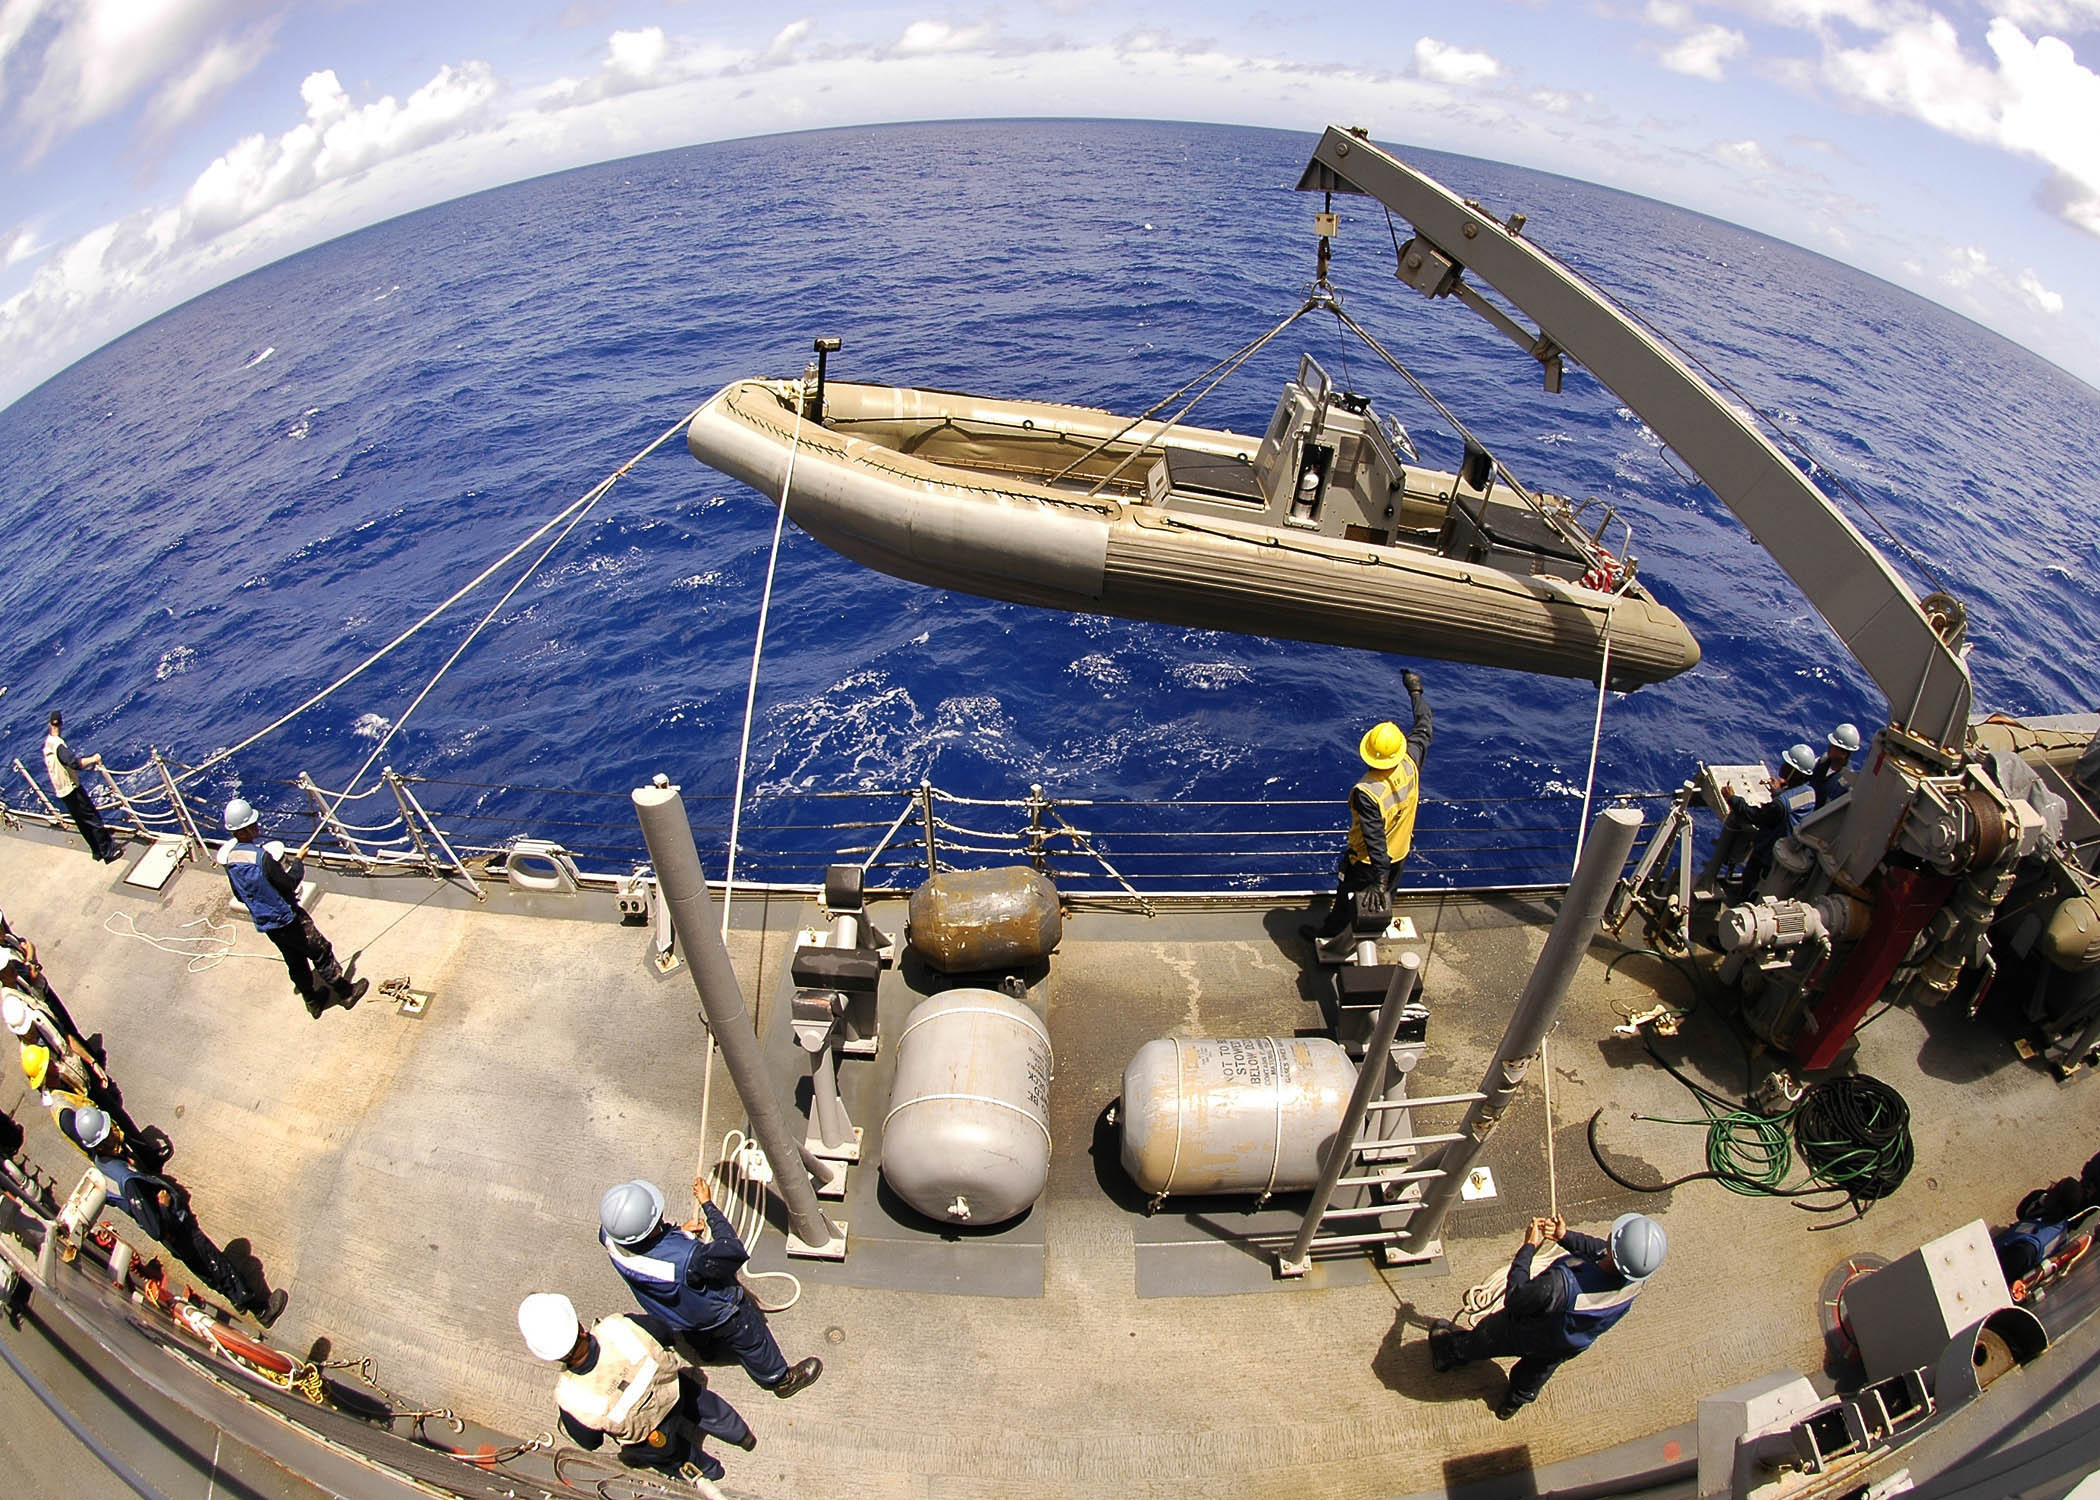
\includegraphics[width=5cm]{navy_rhib.jpg}
        \caption{Sailors launch the Rigid Hull Inflatable Boat (RHIB) aboard the guided-missile destroyer USS Russell (DDG 59). US Navy Released Photo, 060619-N-4166B-009.}
        \label{fig:navy_rhib}
	\end{minipage}
	\hfill
	\begin{minipage}[b]{0.45\textwidth}
		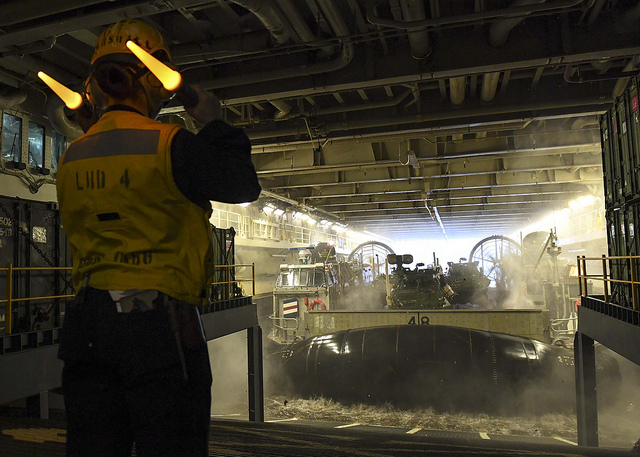
\includegraphics[width=5cm]{lcac.jpg}
        \caption{A landing craft, air cushion (LCAC) is launched from the well deck of the USS Boxer (LHD 4). US Navy Released Photo, 190116-N-SH168-1054.}
        \label{fig:navy_lcac}
	\end{minipage}
\end{figure}

The launch and recovery spaces of a ship can have large impacts on the overall ship design. Some launch and recovery systems will dictate large portions of the ship arrangements and will be primary design drivers such as flight decks, well decks, and stern ramps. Other systems, such as davits and articulating cranes, will have minimal impact on the overall design. This makes the analysis of the design alternatives an important aspect of the overall design process.

\subsection{Bayesian Networks}

Bayesian networks are a type of directed acyclic graph (DAG) encoded with conditional probability distributions. The network allows the expression of relationships which can result in simplified knowledge generation and transparency to relationship dependencies. Bayesian networks allow for both top-down and bottom-up reasoning, which means that the outcome can be predicted, given a set of inputs, or given an outcome, the root cause of the outcome can be identified \cite{murphy_brief_1998}. 

Bayesian networks are directed graphs, meaning they show the directionality of relationships. Bayesian networks rely on the use of Baye's Theorem for Bayesian inference, shown in Equation~\ref{eq:bayes}. The posterior distribution, $P(\theta|y)$, represents the probability that is the basis for action, given collected knowledge, $y$. This utilizes information from a prior distribution, $P(\theta)$, and the likelihood function, $P(y|\theta)$. 

\begin{equation}
    P(\theta|y) = \frac{P(y|\theta)P(\theta)}{P(y)}
    \label{eq:bayes}
\end{equation}

The marginal distribution, $P(y)$, is a normalizing constant that is often disregarded, as it can be difficult to determine \cite{gelman_bayesian_2013}, and the result is that in Bayesian inference we may only show the proportionality of the posterior to the likelihood and prior, shown in Equation~\ref{eq:bayes2}. 

\begin{equation}
    P(\theta|y) \propto {P(y|\theta)P(\theta)}
    \label{eq:bayes2}
\end{equation}

Bayesian networks rely on joint probability distributions to combine parent nodes for the child node. In this probabilistic model, each variable, $X_i$ is represented as a node on the DAG. The probability distribution $P(X_1,X_2,...,X_n)$ is represented as follows:

\begin{equation}
    P(X_1,X_2,...,X_n) = \prod_{i=1}^n P(X_i|\Pi_{X_i})
    \label{eq:conditional_prob}
\end{equation}

\noindent
where $\Pi_{X_i}$ represents the set of nodes tha are the parents to $X_i$ in the network topology. 

Bayesian networks are widely used in engineering and defense research. Bayesian networks have been used to predict drinking water distribution pipe breaks \cite{francis_bayesian_2014}. They have also been used for probabilistic assessments for nuclear waste disposal \cite{lee_application_2006}, and predicting air defense threats \cite{johansson_bayesian_nodate}. In marine structural engineering, they have been used in structural performance and reliability models \cite{groden_fusing_2017}. There have been some limited applications in marine design \cite{friis-hansen_bayesian_2000}, and in marine decision making \cite{eleye-datubo_enabling_2006}. 

In some of these cases, the network topology was learned from the data \cite{francis_bayesian_2014}, while in others it was determined by the authors \cite{johansson_bayesian_nodate}, \cite{groden_fusing_2017}. 

\FloatBarrier 


\section{Methodology}

With no data readily available to train a network structure, the network structure for this methodology is adapted from Wireman, 2019 \cite{wireman_leading_2019}. This model is intended to show the ability of Bayesian Networks to examine a ship design, and does not necessarily try to perfectly model individual variables such as crane operating capacities.  

The previous influence diagram structure was slightly modified. The variables included are described further in Tables~\ref{table:variables} and~\ref{table:variables2}. The full network structure is shown in Figure~\ref{fig:whole_tree}, with the four primary subtrees shown separately in Figures~\ref{fig:host_tree}--\ref{fig:env_tree}. 

All modeling was performed in Python 2.7. All graphing of the networks was performed using the NetworkX, \cite{networkx_2018}, and Graphviz, \cite{graphviz_2018}, packages for Python. 

The model takes in 14 primary input variables, listed in Table~\ref{table:variables}, which are the first nodes below each of the four variable categories. From here, the input nodes are passed to the first layer of calculated intermediate nodes. These intermediate nodes utilize joint conditional probability tables to determine the outcome of the input node. These joint conditional probability tables are shown in Tables~\ref{table:prob_ratings}--\ref{table:prob_crew}.

In instances where the input variable is a rating, Table~\ref{table:prob_ratings} is used to determine the probability that the outcome will be satisfactory. Table~\ref{table:prob_weight} is used for variables where the weight of the launch or recovery vehicle is dependent. Table~\ref{table:prob_volume} is for variables that are dependent on the vehicle volume, Table~\ref{table:prob_fbd} is for variables dependent on the ship freeboard, and Table~\ref{table:prob_crew} is used for variables dependent on the crew size. 

\begin{table}[htb]
\begin{center}
\setlength\extrarowheight{3.5pt}
\caption{Variables included in the Bayesian Network.}
\begin{tabular}{p{3.5cm}  p{8.7cm}}
\hline
Item                          & Description                                                                        \\
\hline
\hline 
Host Vessel                   & The ship that the secondary vehicle is being launched from or recovered onto       \\
Arrangement \linebreak Flexibility*      & Rating of if the ship design's arrangement is flexible                             \\
Crew Size*                     & Total number of crew members on the host vessel                                    \\
Minimum Freeboard*             & Minimum freeboard required for the ship, in meters                                  \\
Available Manning             & Probability there will be enough crew to man the launch/recovery                   \\
\hline
Vehicle                       & The vehicle being launched or recovered                                            \\
Vehicle Volume*                & The volume of the vehicle, in cubic meters                                         \\
Vehicle Weight*                & The weight of the vehicle, in metric tons                                          \\
Variability \linebreak of Vehicle Type*   & Rating of the variability of other vehicles of the same type                       \\
L/R Flexibility*               & Rating of the flexibility the vehicle has for multiple launch/recovery methods     \\
Vehicle Complexity*            & Rating of how complex the vehicle is to launch/recover                             \\
\hline
L/R System                    & The launch or recovery system                                                      \\
System \linebreak Requirements*           & Rating of the overall requirements of the launch/recovery \linebreak system                   \\
Arrangement Impact            & Probability that the system does not heavily impact the ship design's arrangements \\
Required Manning              & Probability that the manning requirement of the system can be satisfied            \\
Freeboard \linebreak Flexibility*         & Rating of the flexibility of the system to deal with various freeboard amounts     \\
Relative Height*               & Rating of how close to the water level or top of the ship the system is            \\
Simplicity of L/R             & Probability that the system will be simple to execute                              \\
Rated Capacity*                & The rated capacity of the system, in metric tons                                   \\
Actual Capacity               & A probabilistically determined capacity of the system                              \\
\hline
Environment                   & The environmental conditions                                                       \\
Sea State Rating*              & Rating of the sea state condition and impact on the launch and recovery            \\
Wind Speeds*                   & Rating of the wind conditions and impact on the launch and recovery                \\
Freeboard Available           & Probability of environmental impacts on the freeboard      \\
\hline
\multicolumn{2}{l}{* Denotes input variables to the network}
\end{tabular}
\label{table:variables}
\end{center}
\end{table}

\begin{table}[htb]
\begin{center}
\setlength\extrarowheight{3.5pt}
\caption{The satisfaction variables included in the Bayesian Network.}
\begin{tabular}{p{3.5cm}  p{8.7cm}}
\hline
Item                          & Description                                                                        \\
\hline
\hline 
Arrangement \linebreak Satisfaction      & Probability that the arrangement of the ship is satisfactory                       \\
Manning\linebreak Satisfaction          & Probability that the manning levels are satisfactory                                \\
Freeboard \linebreak Satisfaction        & Probability that the freeboard levels will be satisfactory                         \\
Performance \linebreak Satisfaction      & Probability that the performance of the launch/recovery will be satisfactory       \\
Interoperability \linebreak Satisfaction & Probability that the interoperability of multiple vehicles will be satisfactory                 \\
Overall Satisfaction          & Overall probability of satisfaction  \\   
\hline
\end{tabular}
\label{table:variables2}
\end{center}
\end{table}

\begin{table}
	\begin{minipage}{0.5\linewidth}
		\caption{The conditional probability table for the rated variables.}
		\label{table:prob_ratings}
		\centering
            \begin{tabular}{c c}
            \hline
            Rating & P(Satisfactory) \\
            \hline
            1      & 0.99            \\
            2      & 0.98            \\
            3      & 0.95            \\
            4      & 0.80            \\
            5      & 0.50            \\
            6      & 0.20            \\
            7      & 0.10            \\
            8      & 0.05            \\
            9      & 0.01  \\
            \hline
            \end{tabular}
	\end{minipage}\hfill
	\begin{minipage}{0.45\linewidth}
		\caption{The conditional probability table for the mass variables.}
		\label{table:prob_weight}
		\centering
            \begin{tabular}{c c}
            \hline
            Mass (mt) & P(Satisfactory) \\
            \hline
            1           & 0.99            \\
            5           & 0.98            \\
            10          & 0.95            \\
            20          & 0.90            \\
            30          & 0.80            \\
            40          & 0.70            \\
            50          & 0.60            \\
            100         & 0.40            \\
            200         & 0.30  \\
            \hline
            \end{tabular}
	\end{minipage}
\end{table}

\begin{table}
	\begin{minipage}{0.5\linewidth}
		\caption{The conditional probability table for the volumetric variables.}
		\label{table:prob_volume}
		\centering
            \begin{tabular}{c c}
            \hline
            Volume (m$^3$) & P(Satisfactory) \\
            \hline
            0.1         & 0.99            \\
            1.0         & 0.95            \\
            5.0         & 0.85            \\
            10.0        & 0.75            \\
            20.0        & 0.55            \\
            30.0        & 0.40            \\
            40.0        & 0.30            \\
            50.0        & 0.22            \\
            75.0        & 0.10            \\
            100.0       & 0.05            \\
            150.0       & 0.01   \\
            \hline
            \end{tabular}
	\end{minipage}\hfill
	\begin{minipage}{0.45\linewidth}
		\caption{The conditional probability table for the freeboard variables.}
		\label{table:prob_fbd}
		\centering
            \begin{tabular}{c c}
            \hline
            Fbd Min (m) & P(Satisfactory) \\
            \hline
            0.5         & 0.99            \\
            1.0         & 0.95            \\
            2.0         & 0.85            \\
            3.0         & 0.75            \\
            4.0         & 0.65            \\
            5.0         & 0.55            \\
            6.0         & 0.45            \\
            7.0         & 0.35            \\
            8.0         & 0.25            \\
            9.0         & 0.15            \\
            10.0        & 0.05  \\
            \hline
            \end{tabular}
	\end{minipage}
\end{table}


\begin{table}[htb]
\begin{center}
\setlength\extrarowheight{3.5pt}
\caption{The conditional probability table for the crew-based variables.}
\begin{tabular}{r c}
\hline
Crew Size & P(Satisfactory) \\
\hline
5         & 0.01            \\
10        & 0.08            \\
15        & 0.15            \\
20        & 0.20            \\
30        & 0.30            \\
40        & 0.40            \\
50        & 0.50            \\
60        & 0.60            \\
80        & 0.72            \\
100       & 0.80            \\
150       & 0.90            \\
200       & 0.95            \\
400       & 0.99            \\
\hline
\end{tabular}
\label{table:prob_crew}
\end{center}
\end{table}

In this method, $P(\theta)$ is the probability of a satisfactory design outcome, given observations $y_i$. There are several intermediate satisfaction metrics, including Freebaord Satisfaction, $\theta_f$, Arrangement Flexibility Satisfaction, $\theta_a$, Manning Satisfaction, $\theta_m$, Peformance Satisfaction, $\theta_p$, and Vehicle Interoperability Satisfaction, $\theta_i$. 

The probability of a satisfactory design outcome was the metric chosen as the key performance indicator to evaluate the overall design effectiveness from the network. This metric could have been any number of things including cost effectiveness or mission effectiveness. This metric was chosen for its simplicity. 

There are multiple intermediate variables which contribute to the knowledge base. In most cases, these are calculated as:

\begin{equation}
    P(\theta_{child}) = \prod_{i=1}^N P(\theta_{parent,i}|y_i)
\end{equation}

\noindent
where the child nodes are the dependent intermediate nodes, and the $N$ parent nodes are the nodes above them in the hierarchy which have edges leading to the child signifying dependence. The parent probabilities are calculated using the conditional probability tables previously described. 

In the case of the probabilistic estimate of the actual capacity of the launch and recovery system, $C_a$, it is calculated as follows:

\begin{equation}
    C_a = C_r - 0.5I
\end{equation}

\noindent
where $C_r$ is the rated capacity, and $I$ is the impact of the other dependent nodes, which is calculated as: 

\begin{equation}
    I = C_r(1-P(\theta|y_{wind})P(\theta|y_{ss}))
\end{equation}

\noindent
where $P(\theta|y_{wind})$ and $P(\theta|y_{ss})$ are the conditional probabilities from the impact of the wind and the sea state, respectively. 

In the case of the Performance Satisfaction, the weight of the vehicle needs to be considered compared to the actual capacity of the launch and recovery system. In this case, the probability of satisfaction is calculated as follows:

\begin{equation}
    P(\theta_p) = 
    \begin{cases}
    0.01,& \text{if } W > C_a\\
    P(\theta|y_{cmplx})((1-W/C_a) + 0.25),              & \text{otherwise}
\end{cases}
\end{equation}

\noindent
where W is the weight of the vehicle, $P(\theta|y_{cmplx})$ is the probability of satisfaction given the complexity of the vehicle, and $((1-W/C_a) + 0.25)$ is capped at 1.0. 

The overall satisfaction, $P(\theta)$, is computed as the geometric mean of $P(\theta_{f,a,m,p,i})$:

\begin{equation}
    P(\theta) = [P(\theta_f)P(\theta_a)P(\theta_m)P(\theta_p)P(\theta_i)]^{1/5}
\end{equation}

\begin{figure}[htb]
\begin{adjustwidth}{-0.5cm}{-.5cm} 
\centering
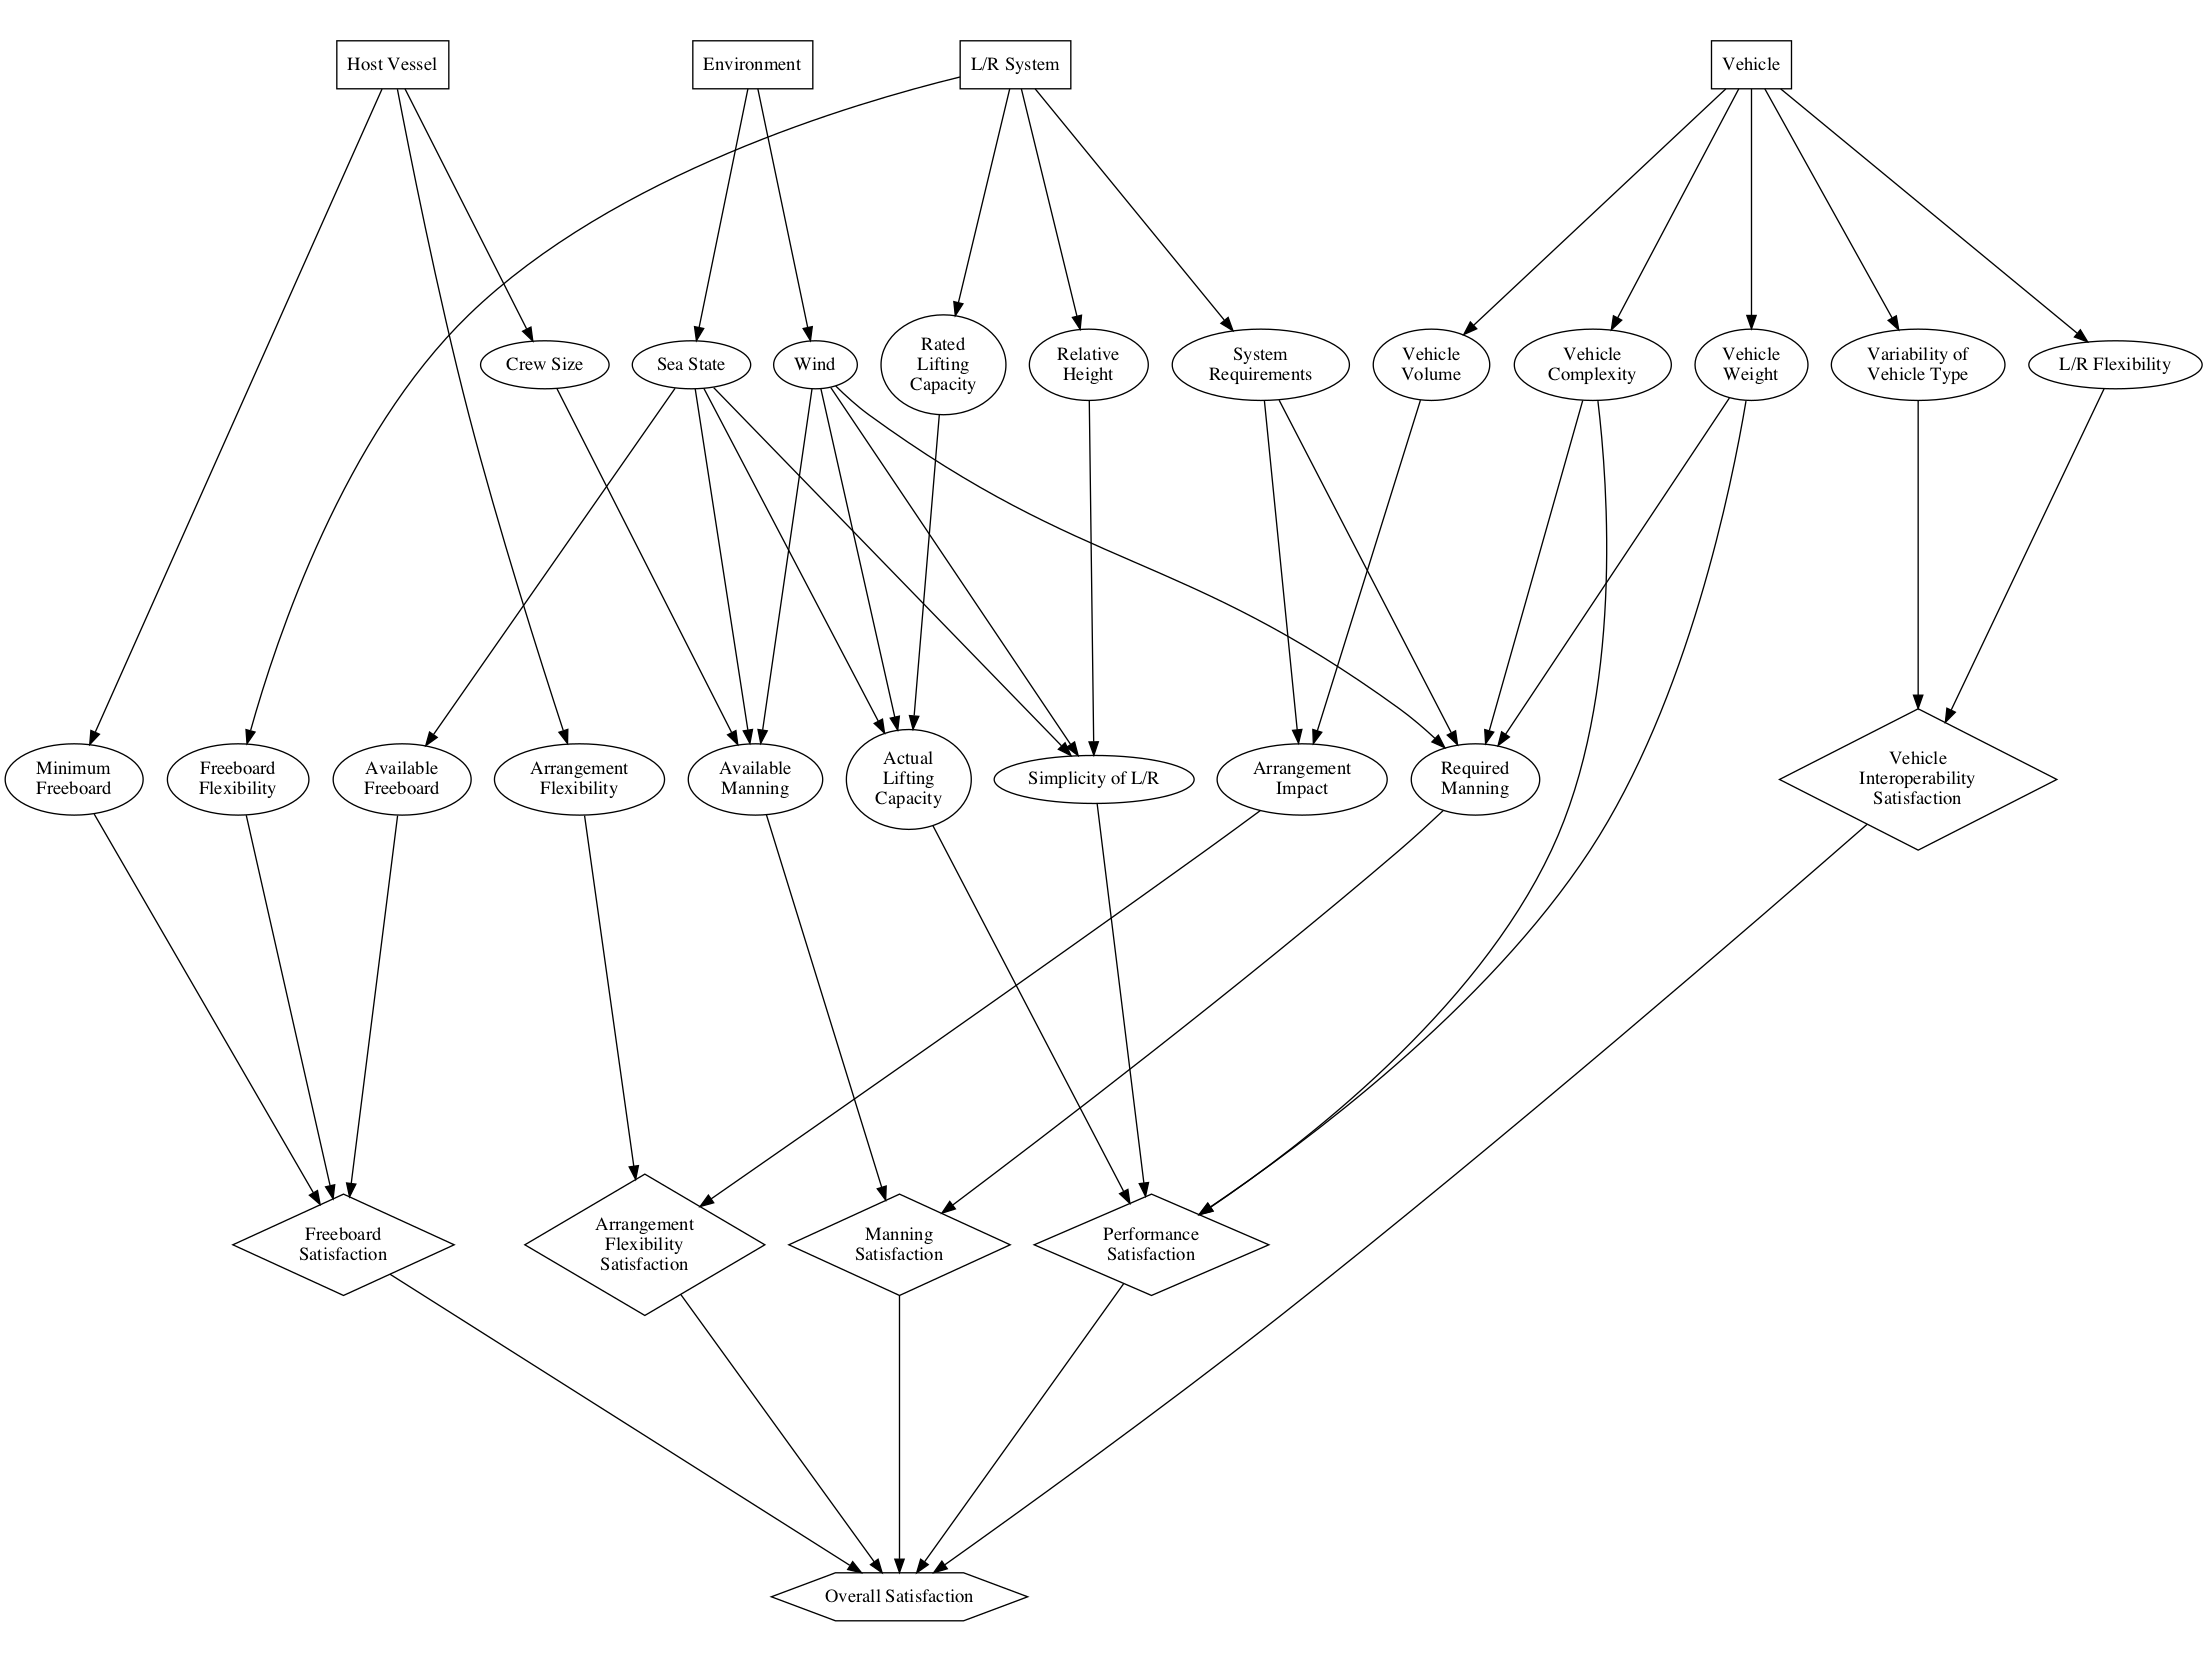
\includegraphics[width=13.2cm]{whole_tree.png}
\caption{The full network tree developed. Closer views of the four primary subtrees are shown in Figures~\ref{fig:host_tree},~\ref{fig:vehicle_tree},~\ref{fig:system_tree}, and~\ref{fig:env_tree}.}
\label{fig:whole_tree}
\end{adjustwidth} 
\end{figure}

\begin{figure}[htb]
\begin{adjustwidth}{-0.5cm}{-.5cm} 
\centering
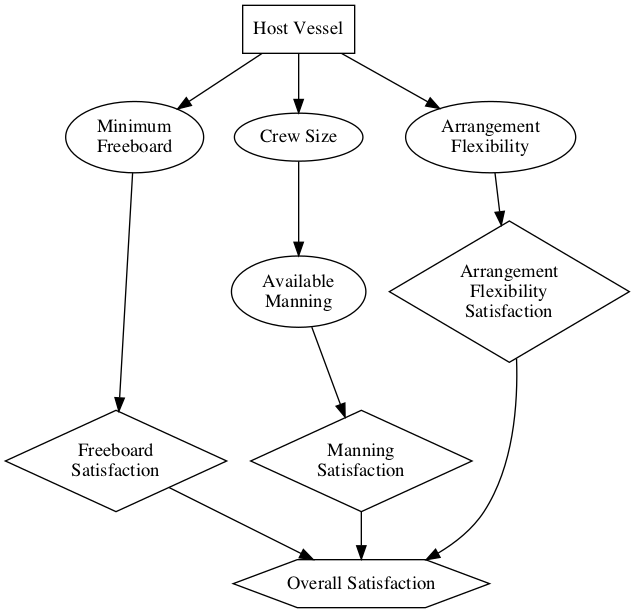
\includegraphics[width=10cm]{host_vessel_tree.png}
\caption{The Host Vessel portion of the network is shown.}
\label{fig:host_tree}
\end{adjustwidth} 
\end{figure}

\begin{figure}[htb]
\begin{adjustwidth}{-0.5cm}{-.5cm} 
\centering
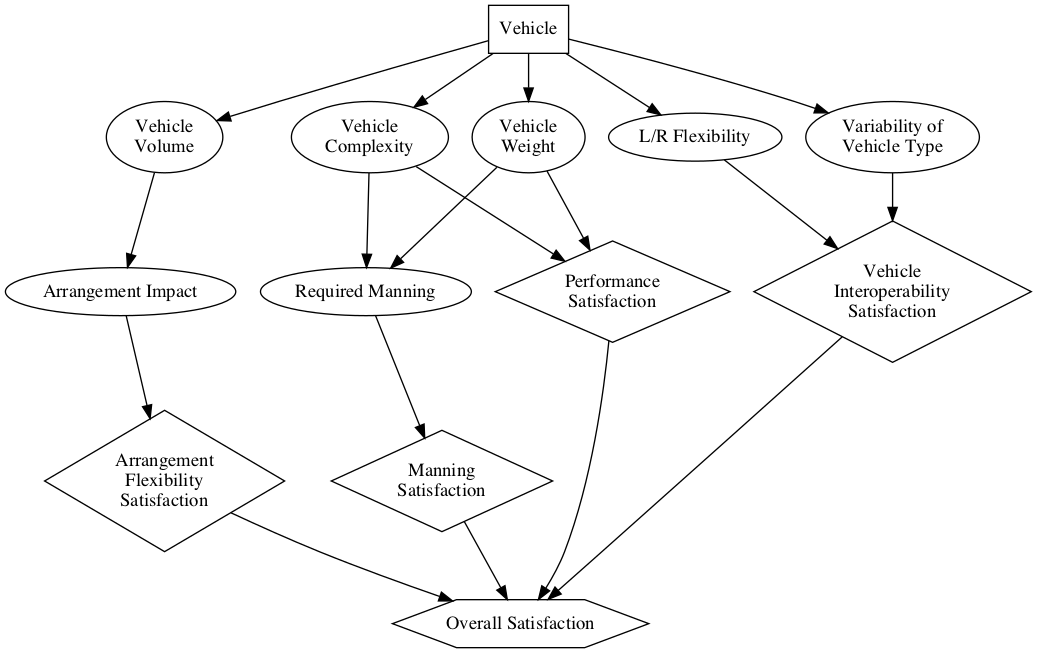
\includegraphics[width=13.2cm]{vehicle_tree.png}
\caption{The Vehicle portion of the network is shown.}
\label{fig:vehicle_tree}
\end{adjustwidth} 
\end{figure}

\begin{figure}[htb]
\begin{adjustwidth}{-0.5cm}{-.5cm} 
\centering
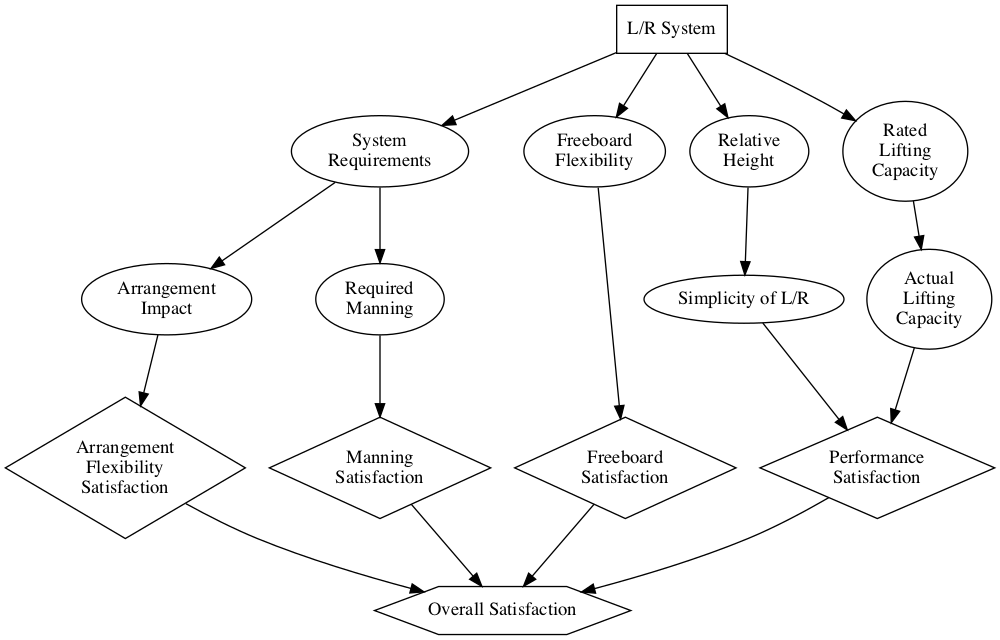
\includegraphics[width=13.2cm]{system_tree.png}
\caption{The Launch and Recovery System portion of the network is shown.}
\label{fig:system_tree}
\end{adjustwidth} 
\end{figure}

\begin{figure}[htb]
\begin{adjustwidth}{-0.5cm}{-.5cm} 
\centering
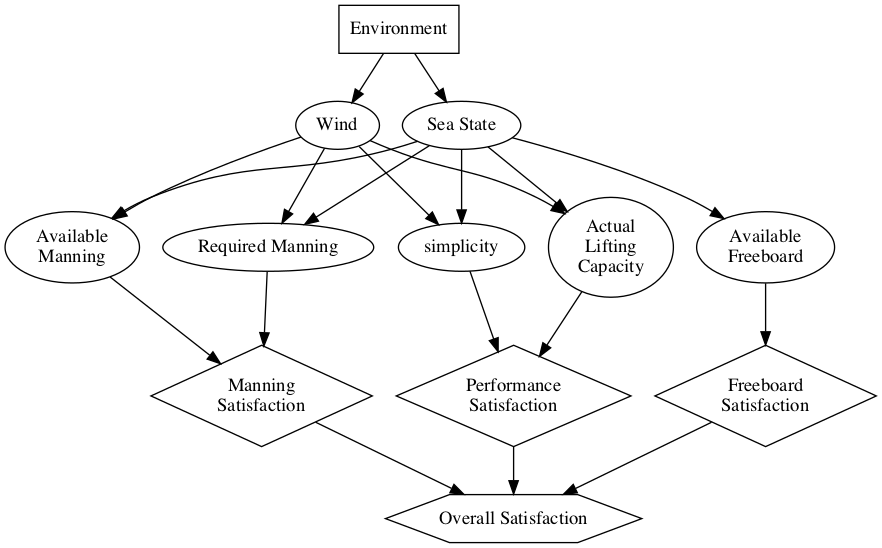
\includegraphics[width=13.2cm]{env_tree.png}
\caption{The Environmental portion of the network is shown.}
\label{fig:env_tree}
\end{adjustwidth} 
\end{figure}

\FloatBarrier

\section{Model Sensitivity}

To examine the effectiveness of the proposed model, a simple sensitivity analysis is examined. A sample hose vessel, vehicle, launch and recovery system, and environmental conditions are proposed. From this baseline, each variable is changed independent of the rest between the  minimum and maximum values assessed in the conditional probability tables. The baseline input variables, as well as the maximum and minimum values, are shown in Table~\ref{table:input}. 

\begin{table}[htb]
\begin{center}
% \setlength\extrarowheight{1pt}
\caption{The input variables for the case study. The baseline value is shown along with the minimum and maximum values used in the simulation.}
\begin{tabular}{l l r r r}
\hline
 & Input Variable & & Value                &     \\
               &                         & Baseline & Min & Max \\
\hline
Host Ship      & Arrangement Flexibility & 3    & 1   & 9   \\
               & Crew Size               & 200  & 5   & 400 \\
               & Freeboard Minimum       & 1    & 1   & 9   \\
Vehicle        & Volume [m$^3$]          & 15   & 0.1 & 150 \\
               & Weight [mt]             & 20   & 0.5 & 200 \\
               & Variability             & 3    & 1   & 9   \\
               & Flexibility             & 3    & 1   & 9   \\
               & Complexity              & 2    & 1   & 9   \\
L/R System     & System Requirements     & 2    & 1   & 9   \\
               & Freeboard Flexibility   & 2    & 1   & 9   \\
               & Relative Height         & 2    & 1   & 9   \\
               & Capacity [mt]           & 40   & 0.5 & 300 \\
Environment    & Sea State               & 2    & 1   & 9   \\
               & Wind                    & 2    & 1   & 9   \\
\hline
\end{tabular}
\label{table:input}
\end{center}
\end{table}

The baseline variable selection results in an overall probability of satisfaction of 0.76. This is reflected in Figure~\ref{fig:baseline} and Table~\ref{table:baseline}. As shown, under the baseline conditions the overall satisfaction is being driven positively by the vehicle interoperability and is being driven negatively by the manning requirement. 

\begin{figure}[!htb]
\centering
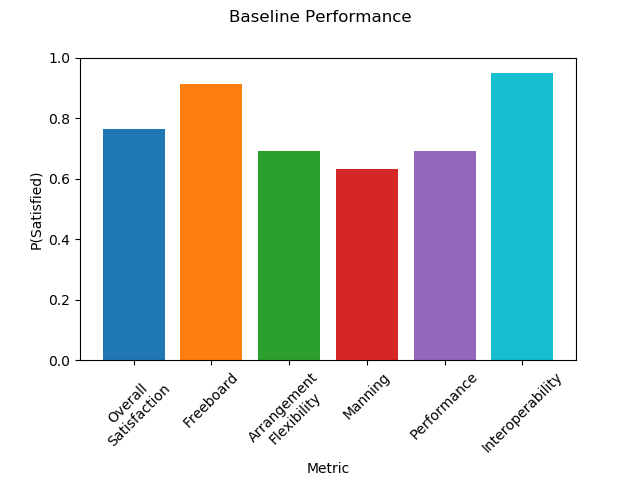
\includegraphics[width=9cm]{baseline.png}
\caption{The baseline performance data from the initial simulation. The overall satisfaction is 0.76, which is largely driven down by the poor probability of manning satisfaction, arrangement flexibility, and performance.}
\label{fig:baseline}
\end{figure}

\newcolumntype{P}[1]{>{\centering\arraybackslash}p{#1}}

\begin{table}[!htb]
\begin{center}
% \setlength\extrarowheight{1pt}
\caption{The results of the baseline variables through the network.}
\begin{tabular}{P{2cm} P{2cm}}
\hline
Variable & Value \\
\hline
$P(\theta)$        & 0.76  \\
$P(\theta_f)$        & 0.91  \\
$P(\theta_a)$       & 0.69  \\
$P(\theta_m)$       & 0.63  \\
$P(\theta_p)$        & 0.69  \\
$P(\theta_i)$       & 0.95  \\
\hline
\end{tabular}
\label{table:baseline}
\end{center}
\end{table}

Using this baseline data as a starting point, 134 test cases are simulated by varying each input variable independently. From this data, the most useful data was determined to be the maximum, minimum, and the difference between the maximum and minimum values for each of the satisfaction probabilities. This data is shown in Table~\ref{table:min_max} and Table~\ref{table:diff}.  

\begin{table}[!htb]
\begin{adjustwidth}{-0.5cm}{-.5cm}
\begin{center}
% \setlength\extrarowheight{1pt}
\caption{The minimum and maximum results from the simulation.}
\begin{tabular}{l | c c c c c c | c c c c c c}
\hline
\multicolumn{1}{c}{Input Variable} & \multicolumn{6}{c}{Minimum Output}         &      \multicolumn{6}{c}{Maximum Output} \\
& $P(\theta)$ & $P(\theta_f)$ & $P(\theta_a)$ & $P(\theta_m)$ & $P(\theta_p)$ & $P(\theta_i)$  & $P(\theta)$& $P(\theta_f)$ & $P(\theta_a)$ & $P(\theta_m)$ & $P(\theta_p)$ & $P(\theta_i)$ \\
\hline
Arr Flexibility & 0.31 & 0.91 & 0.01 & 0.63 & 0.69 & 0.95           & 0.77 & 0.91 & 0.72 & 0.63 & 0.69 & 0.95 \\
Crew Size               & 0.31 & 0.91 & 0.69 & 0.01 & 0.69 & 0.95           & 0.77 & 0.91 & 0.69 & 0.66 & 0.69 & 0.95 \\
Fbd Minimum       & 0.53 & 0.14 & 0.69 & 0.63 & 0.69 & 0.95           & 0.76 & 0.91 & 0.69 & 0.63 & 0.69 & 0.95 \\
Volume                  & 0.75 & 0.91 & 0.61 & 0.63 & 0.69 & 0.95           & 0.78 & 0.91 & 0.76 & 0.63 & 0.69 & 0.95 \\
Weight                  & 0.26 & 0.91 & 0.69 & 0.21 & 0.01 & 0.95           & 0.83 & 0.91 & 0.69 & 0.69 & 0.92 & 0.95 \\
Variability             & 0.56 & 0.91 & 0.69 & 0.63 & 0.69 & 0.20           & 0.77 & 0.91 & 0.69 & 0.63 & 0.69 & 0.98 \\
Flexibility             & 0.56 & 0.91 & 0.69 & 0.63 & 0.69 & 0.20           & 0.77 & 0.91 & 0.69 & 0.63 & 0.69 & 0.98 \\
Complexity              & 0.31 & 0.91 & 0.69 & 0.63 & 0.01 & 0.95           & 0.77 & 0.91 & 0.69 & 0.63 & 0.70 & 0.95 \\
Sys Requirements     & 0.12 & 0.91 & 0.01 & 0.01 & 0.69 & 0.95           & 0.85 & 0.91 & 0.94 & 0.78 & 0.69 & 0.95 \\
Fbd Flexibility   & 0.34 & 0.01 & 0.92 & 0.77 & 0.69 & 0.95           & 0.85 & 0.92 & 0.92 & 0.77 & 0.69 & 0.95 \\
Relative Height         & 0.34 & 0.91 & 0.92 & 0.77 & 0.01 & 0.95           & 0.85 & 0.91 & 0.92 & 0.77 & 0.70 & 0.95 \\
Capacity                & 0.36 & 0.91 & 0.92 & 0.77 & 0.01 & 0.95           & 0.89 & 0.91 & 0.92 & 0.77 & 0.92 & 0.95 \\
Sea State               & 0.02 & 0.01 & 0.69 & 0.00 & 0.01 & 0.95           & 0.77 & 0.92 & 0.69 & 0.64 & 0.70 & 0.95 \\
Wind                    & 0.05 & 0.91 & 0.69 & 0.00 & 0.01 & 0.95           & 0.77 & 0.91 & 0.69 & 0.64 & 0.70 & 0.95 \\
\hline
\end{tabular}
\label{table:min_max}
\end{center}
\end{adjustwidth} 
\end{table}

\begin{table}[!htb]
\begin{adjustwidth}{-0.5cm}{-.5cm}
\begin{center}
% \setlength\extrarowheight{1pt}
\caption{The difference between the minimum and maximum results of the simulation. A zero indicates that the input variable has no influence on the output.}
\begin{tabular}{l l | c c c c c c}
\hline
\multicolumn{2}{c}{Input Variable} & \multicolumn{6}{c}{Max-Min}         \\
& & $P(\theta)$ & $P(\theta_f)$ & $P(\theta_a)$ & $P(\theta_m)$ & $P(\theta_p)$ & $P(\theta_i)$\\
\hline
Host Ship   & Arrangement Flexibility & 0.46 & 0.00 & 0.71 & 0.00 & 0.00 & 0.00 \\
            & Crew Size               & 0.46 & 0.00 & 0.00 & 0.65 & 0.00 & 0.00 \\
            & Freeboard Minimum       & 0.24 & 0.77 & 0.00 & 0.00 & 0.00 & 0.00 \\
Vehicle     & Volume                  & 0.03 & 0.00 & 0.15 & 0.00 & 0.00 & 0.00 \\
            & Weight                  & 0.56 & 0.00 & 0.00 & 0.48 & 0.91 & 0.00 \\
            & Variability             & 0.21 & 0.00 & 0.00 & 0.00 & 0.00 & 0.78 \\
            & Flexibility             & 0.21 & 0.00 & 0.00 & 0.00 & 0.00 & 0.78 \\
            & Complexity              & 0.46 & 0.00 & 0.00 & 0.00 & 0.69 & 0.00 \\
L/R System  & System Requirements     & 0.73 & 0.00 & 0.93 & 0.77 & 0.00 & 0.00 \\
            & Freeboard Flexibility   & 0.51 & 0.91 & 0.00 & 0.00 & 0.00 & 0.00 \\
            & Relative Height         & 0.51 & 0.00 & 0.00 & 0.00 & 0.69 & 0.00 \\
            & Capacity                & 0.53 & 0.00 & 0.00 & 0.00 & 0.91 & 0.00 \\
Environment & Sea State               & 0.75 & 0.91 & 0.00 & 0.64 & 0.69 & 0.00 \\
            & Wind                    & 0.72 & 0.00 & 0.00 & 0.64 & 0.69 & 0.00 \\
\hline
\end{tabular}
\label{table:diff}
\end{center}
\end{adjustwidth} 
\end{table}

We can validate the model by examining the edge cases. Conceptually, if the sea state is extremely large, the probability of a positive outcome with high satisfaction is low. 

This is accurately depicted in Table~\ref{table:min_max}, where $\text{min}(P(\theta)) = 0.02$ corresponds to the worst sea state condition. Similarly, not having enough crew to perform the task, having extreme system requirements, having a very complex vehicle, or having a heavy vehicle with a medium capacity launch/recovery system all result in low probabilities of satisfaction. This makes sense given our intuition. 

Conversely, we can see improvements over the baseline across the board as we loosen restrictions on the maximum value side of Table~\ref{table:min_max}. Many variables were already near their best case scenarios in the baseline, so only minimal gains were observed. However in the cases of the variables where the baseline was of moderate difficulty (vehicle weight, launch system capacity), larger changes were observed, as expected. In no case do we expect a perfect situation, given the rest of the baseline variables, which is why the overall satisfaction is never expected above 0.89. 

These data allow the identification of the key variables in the design by examining the differences between their minimum and maximum values across the various metrics, shown in Table~\ref{table:diff}. A result of zero indicates that the variable has no influence on the predicted satisfaction. A low number indicates it has low impact, and a high number indicates that it has a large impact. In this case, the data show that the environment has the largest impact on the overall design satisfaction outcome. 

The sea state influences more aspects of the satisfaction outcome than any other element. This is due to the sea state's influence across the board on operations. As the sea state intensifies, ship motions increase and situations can potentially become more dangerous. The safe working load for cranes can be diminished and higher manpower levels can be required for shipboard operations. While individual ships set manning requirements for given ship operations\cite{gayle_analysis_2006}, these can often be increased in heavier sea conditions. 

The volume of the vehicle on the other hand, influences the outcome satisfaction least, through its impact on the arrangement flexibility. While moving a small man-portable UUV can be simple and have no impact on the arrangement flexibility, moving a large helicopter will have a larger impact. However, this larger vehicle will also require a larger launch and recovery system, which is being accounted for in the system requirements side of the arrangement impacts as well. 
The influence paths of these variables are highlighted in Figure~\ref{fig:colored_tree}. 

\begin{figure}[!htb]
\begin{adjustwidth}{-0.5cm}{-.5cm} 
\centering
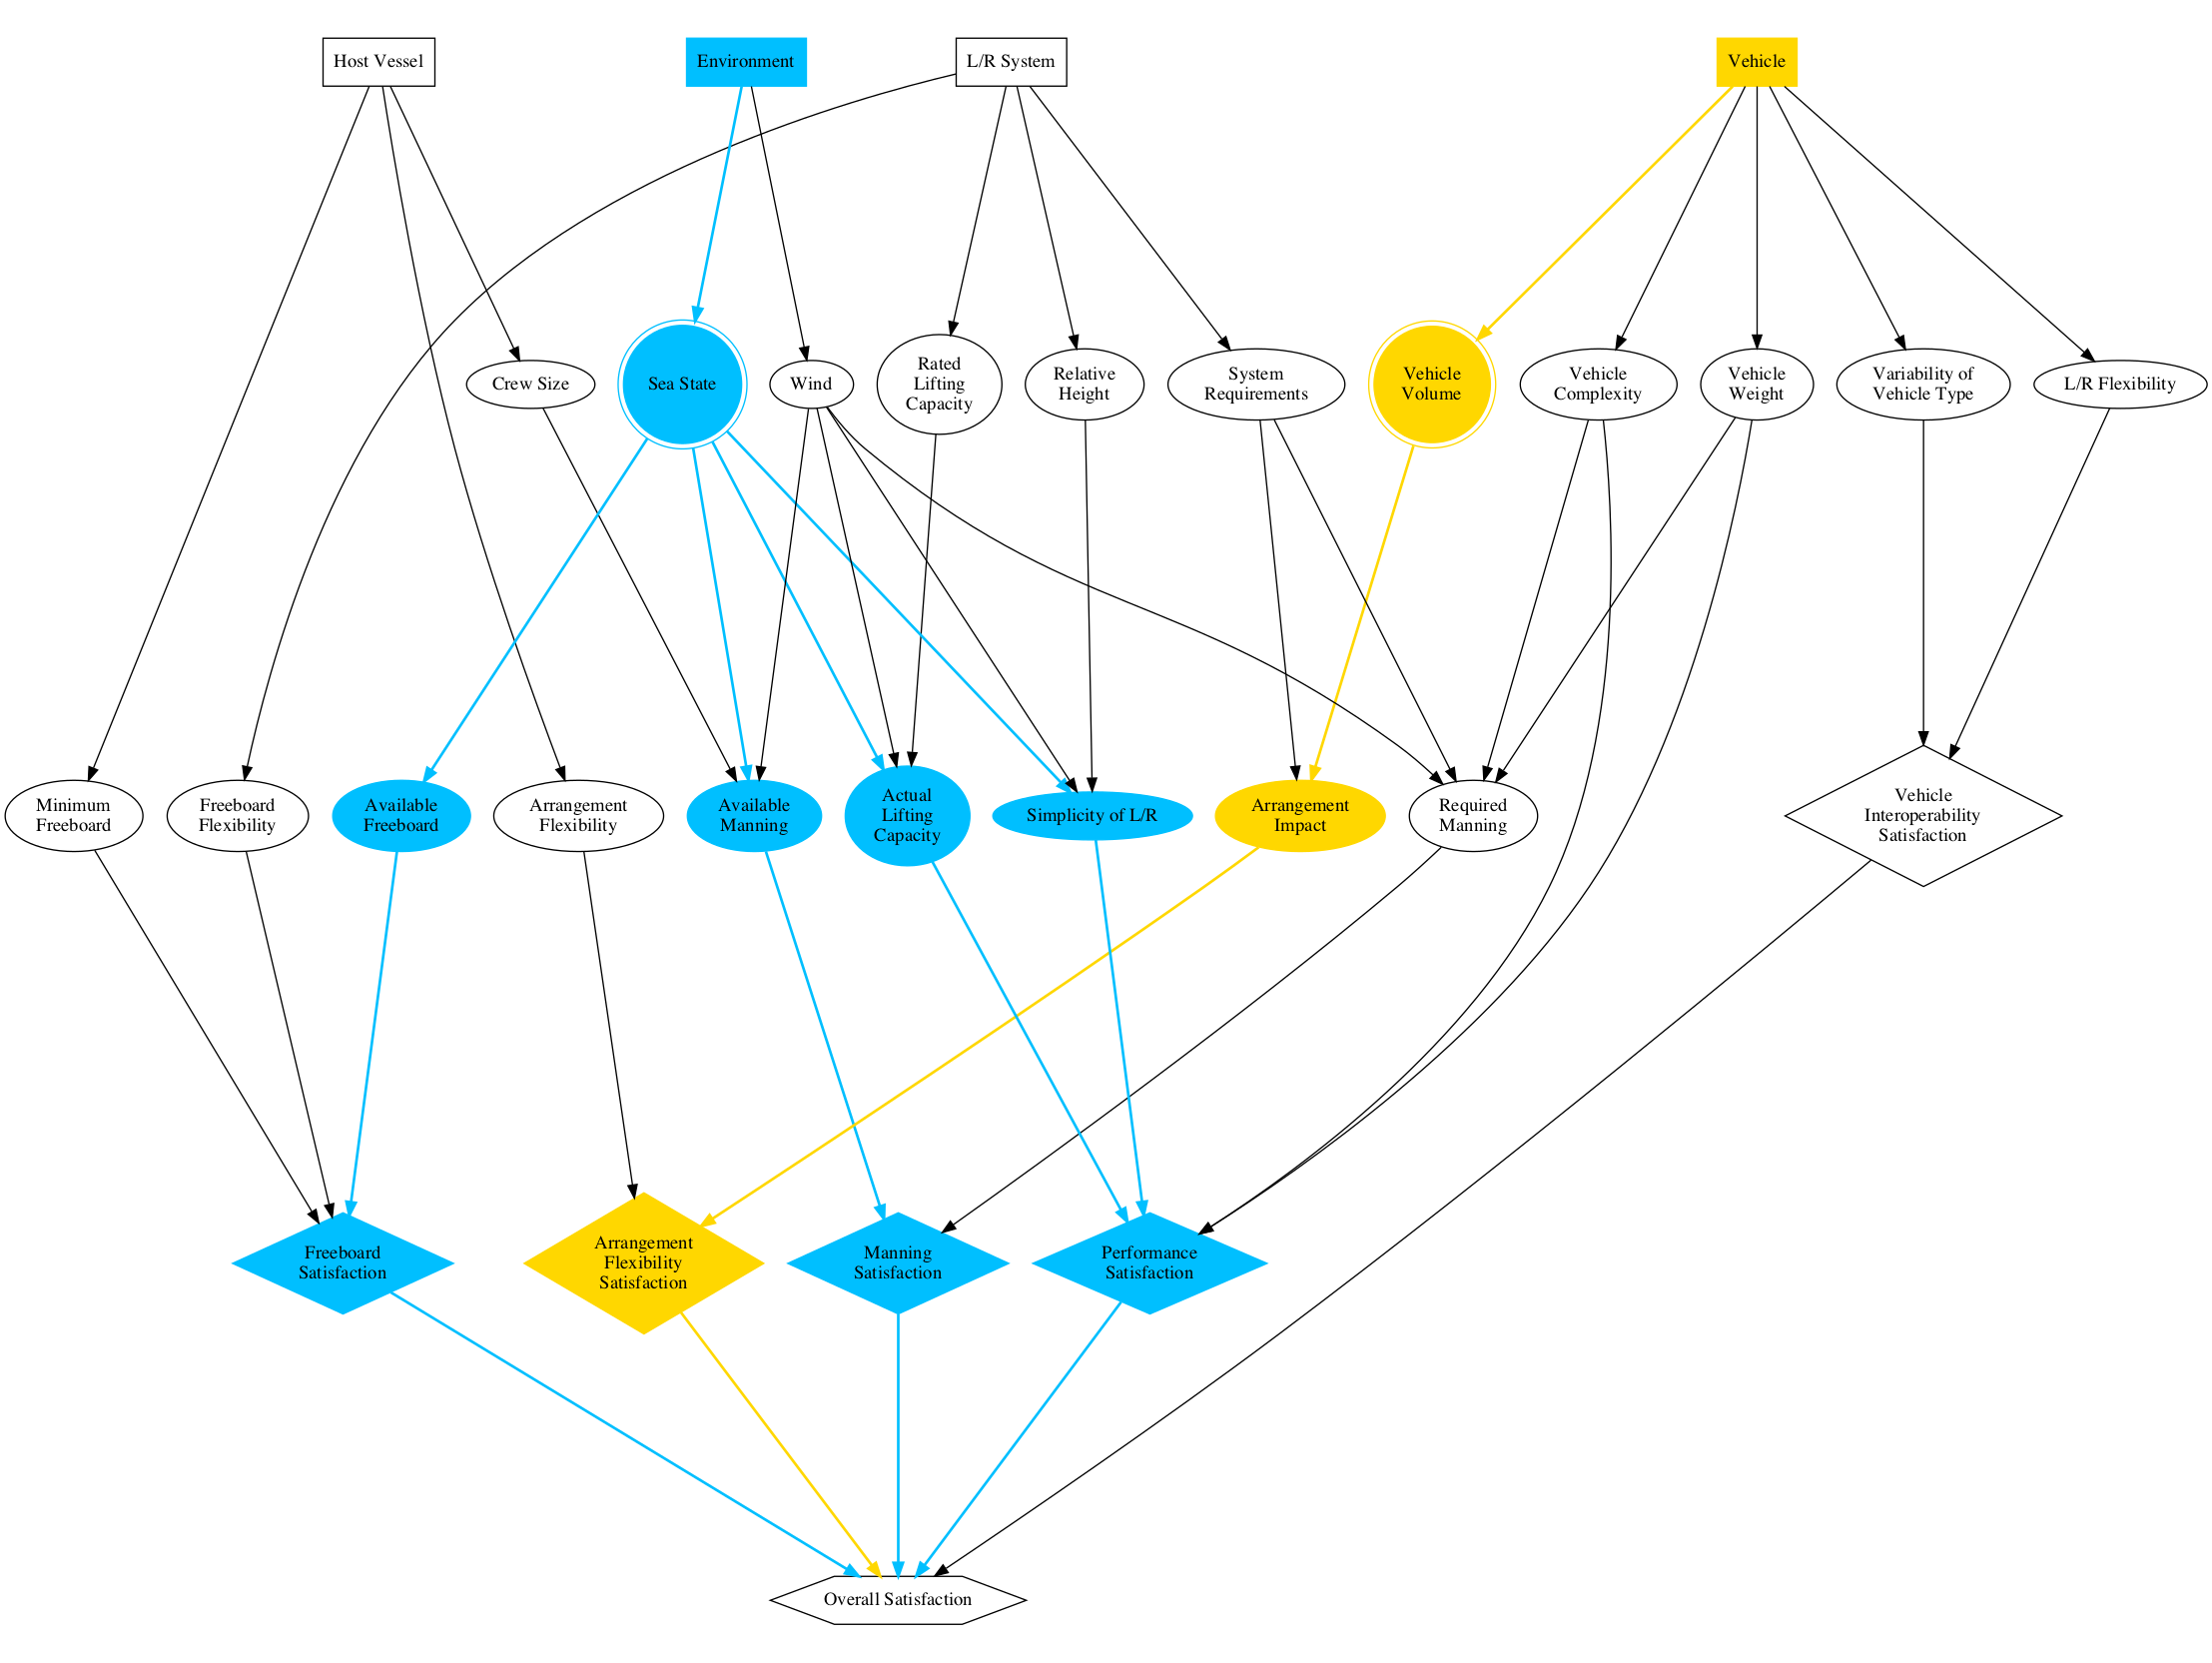
\includegraphics[width=13.2cm]{colored_tree.png}
\caption{The impact of the sea state is (blue path) is high due to its high degree of connectivity. The vehicle volume (yellow path) has very little impact due to its linear path.}
\label{fig:colored_tree}
\end{adjustwidth} 
\end{figure}

The largest impact variable, the sea state, is examined in Figure~\ref{fig:ss1} and Figure~\ref{fig:ss2}. This shows that the overall output function changes with the sea state's conditional probability function, as expected. They do not match exactly because other variables are still influencing the outcome. We can also observe in the data that the sea state does not influence the vehicle interoperability or the arrangement flexibility satisfaction levels since they do not share conditional dependencies, also observable in Figure~\ref{fig:colored_tree}. 

\begin{figure}[hbt]
	\centering
	\begin{minipage}[b]{0.45\textwidth}
		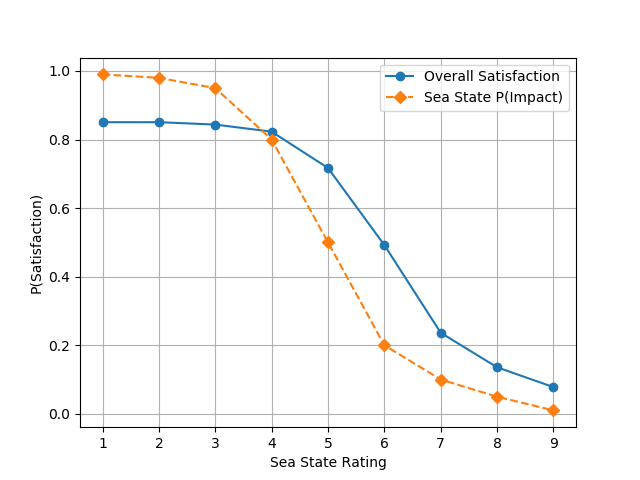
\includegraphics[width=6cm]{ss_plot.png}
        \caption{The sea state's conditional probability function impacts the overall satisfaction due to its heavy influence in the design satisfaction across multiple paths.}
        \label{fig:ss1}
	\end{minipage}
	\hfill
	\begin{minipage}[b]{0.45\textwidth}
		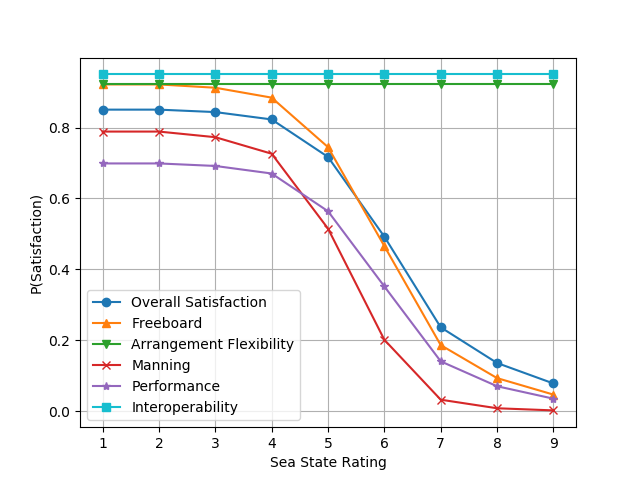
\includegraphics[width=6cm]{ss_plot_2.png}
        \caption{The sea state does not effect the vehicle interoperability or the arrangement flexibility satisfaction levels since they do not share conditional dependencies.}
        \label{fig:ss2}
	\end{minipage}
\end{figure}

\FloatBarrier

\section{Case Study}

In order to examine potential uses of Bayesian networks for early stage ship design, a simple case study is examined. 

In this case study, a ship design has been selected. The ship has an arrangement flexibility score of 3 out of 9, a 100 person crew, and 1 meter of minimum freeboard. The design will integrate one of two crane systems shown in Table~\ref{table:case_cranes}. The two cranes differ in their requirements and capacities. The design is required to integrate three possible vehicles for launch and recovery. The parameters of these three vehicles are listed in Table~\ref{table:case_vehicles}. The three vehicles are a small unmanned underwater vehicle (UUV), a medium duty rigid hull inflatable boat (RHIB) and a heavy duty RHIB. 

\begin{table}[!htb]
\begin{center}
% \setlength\extrarowheight{1pt}
\caption{The variable input values for the two crane systems considered for the case study.}
\begin{tabular}{l r r}
\hline
Variable              & System 1 & System 2 \\
\hline
System Requirements   & 2        & 4        \\
Freeboard Flexibility & 2        & 4        \\
Relative Height       & 2        & 4        \\
Rated Capacity [mt]   & 20       & 40       \\
\hline
\end{tabular}
\label{table:case_cranes}
\end{center}
\end{table}

\begin{table}[!htb]
\begin{center}
% \setlength\extrarowheight{1pt}
\caption{The variable input values for the three vehicles considered for the case study.}
\begin{tabular}{l r r r}
\hline
Variable        & Small UUV & Medium RHIB & Heavy RHIB \\
\hline
Volume {[m$^3$]}& 0.5       & 10          & 15         \\
Weight {[mt]}   & 0.1       & 5           & 10         \\
Variability     & 2         & 4           & 4          \\
Flexibility     & 2         & 3           & 5          \\
Complexity      & 4         & 2           & 3          \\
\hline
\end{tabular}
\label{table:case_vehicles}
\end{center}
\end{table}

\begin{figure}[hbt]
	\centering
	\begin{minipage}[b]{0.45\textwidth}
        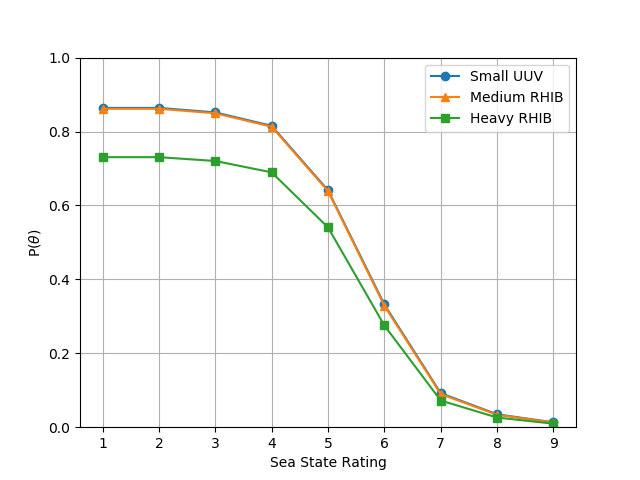
\includegraphics[width=6cm]{case_study_1.png}
        \caption{The results of the case study simulation for crane system 1. The Small UUV and Medium RHIB track almost identically, while the Heavy RHIB has approximately a 10-13\% lower predicted performance satisfaction for Sea State Ratings of 1-5.}
        \label{fig:case1}
	\end{minipage}
	\hfill
	\begin{minipage}[b]{0.45\textwidth}
        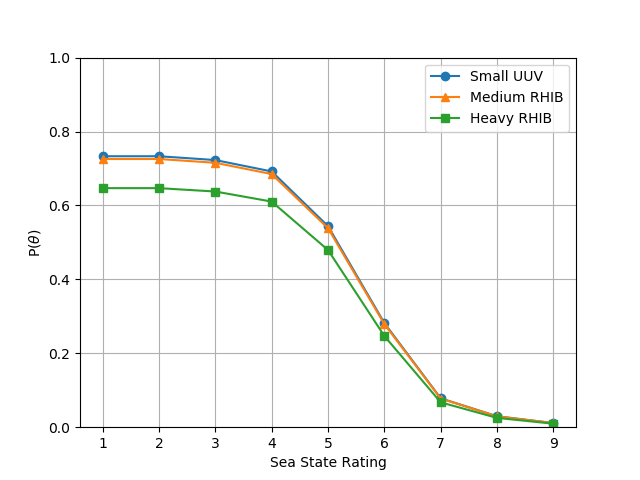
\includegraphics[width=6cm]{case_study_2.png}
        \caption{The results of the case study simulation for crane system 2. The Small UUV and Medium RHIB track almost identically, while the Heavy RHIB has approximately a 10-13\% lower predicted performance satisfaction for Sea State Ratings of 1-5.}
        \label{fig:case2}
	\end{minipage}
\end{figure}

\begin{figure}[htb]
\begin{adjustwidth}{-0.5cm}{-.5cm} 
\centering
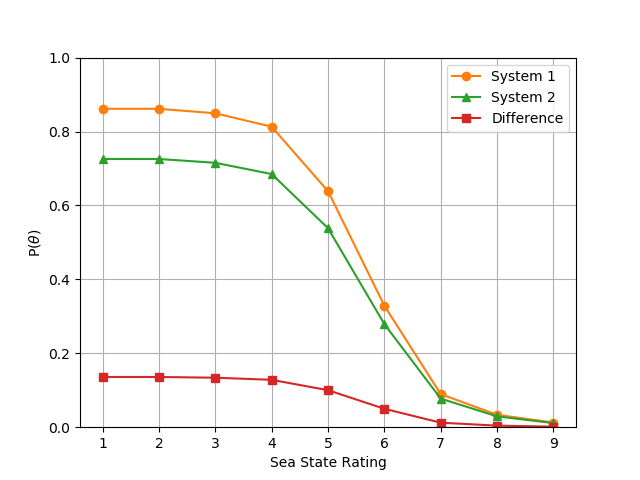
\includegraphics[width=10cm]{case_study_6.png}
\caption{The predicted performance for crane system 1 and crane system 2 are compared for the medium duty RHIB. The difference in performance is also plotted. System 1 has a higher predicted performance satisfaction, with a 13\% difference in lower sea state ratings.}
\label{fig:case_comp}
\end{adjustwidth} 
\end{figure}

In order to quantify the differences between the two launch and recovery systems, the network is simulated for both launch and recovery systems across the three vehicles in nine environmental conditions. In each environmental condition, the sea state and wind rating match one another. 

The results of the two launch systems are shown in Figures~\ref{fig:case1} and~\ref{fig:case2}. As expected from the results of the sensitivity analysis, the overall trend follows that of the environmental condition conditional probability distribution. Of note, this analysis allows the designer to observe that despite differences, the small UUV and medium duty RHIB have an almost identical expected satisfaction probability. The small UUV only has an approximately 2\% advantage over the medium duty RHIB. The heavy duty RHIB's expected performance satisfaction is approximately 15\% lower than the medium duty RHIB.  

In Figure~\ref{fig:case_comp}, the medium duty RHIB case for each launch system is compared, with the difference between them plotted. System 1 has a higher predicted performance satisfaction, with a 13\% difference in lower sea state ratings. As the sea state rating increases, the expected performance satisfaction for both trends toward zero as the likelihood of a successful launch and recovery goes to zero due to the heavy seas. 

By using the Bayesian network, the designer can quantify the differences between potential design choices. A key advantage of the Bayesian network is that the designer can also identify the design drivers of these differences. By using Table~\ref{table:diff} and the differences between the two systems, we can identify the overall system requirements as the driving factor to differentiate the two systems. The Bayesian network allows us to understand that amongst the numerous interdependencies, the system requirements vary the most between the systems and has the potential to have a large impact. 

Further, in investigating the differences between the vehicles, we can identify the vehicle weight as the most likely factor driving the expected probability of design satisfaction since it impacts a large portion of the tree. 

Overall, this method has allowed the designer to quantify the design differences and visualize and recognize the design factors that are driving these differences. 


\FloatBarrier

\section{Analysis} 

This model is extremely simplified, but it shows that a Bayesian network structure can be effective in a ship design case. This model was intended to show that Bayesian networks can be used in quantifying uncertainty in early stage design, and it has shown that. The model outcome is heavily dependent upon both the conditional probability tables as well as the network structure, so it is no surprise that in this simulated model the outcomes were predicable given our knowledge of the underlying assumptions. 

In this case, no real data was available to train a network structure and create the conditional probability tables through learning algorithms. Algorithms exist that will allow the network structure to be built up from provided input data, based on observed dependencies. Francis, 2014 \cite{francis_bayesian_2014} is an example of this.

One major problem with a ship design Bayesian network model is that the variables are all very dependant upon one another. Ship design is a complex problem, sometimes referred to as a ``wicked problem'' \cite{andrews_comprehensive_1998}. The ship design, vehicle, launch and recovery system, and environmental impacts are not readily decomposed.  Because of the lack of decomposition one needs to be cautious that the structure of the network does not lead to interdependent outcomes that are heavily impacted on single variable changes. 

The advantage of this structure is that it can allow these interdependencies to be visualized and quantified. While a designer may realize that the choice in locating a davit on deck 3 versus deck 5 may have an impact on the launch and recovery operation for a RHIB, by examining those decision trade-offs in a properly calibrated Bayesian network, the trade space can be quantified. Additional interdependencies that may not have been immediately realized can be quickly observed and quantified. 

\section{Conclusion}

Identifying and quantifying the impact of design choices within a ship design program is critical for the success of the design. Simple early stage design tools with minimal computational cost are critical in order to evaluate these design decisions. 

In this paper, a simple Bayesian network structure was developed to evaluate the performance of a shipboard launch and recovery operation. A sensitivity analysis of the network structure, which is novel within the Bayesian network literature, and a case study, were developed which provided insight into both the network structure and design decision making has been presented. 

Future work in this area can extend the Bayesian network to other use cases in ship design such as examining a general arrangement layout, integrating ship fleets, or modeling casualty response in damage conditions. Other research work is also being performed to examine the use of Bayesian networks in design optimization. An extension of this work can also incorporate uncertainty in design to understand the impact of the uncertainty in decision making. Additional factors can be included in future analysis, including cost, which has a large impact on ship acquisition. 

The Bayesian network allows for increased transparency and knowledge generation in the design process. Interdependencies can be visualized and quantified through probabilistic methods. 

While limited, the results of this study justify further research in the area of modeling uncertainty and the decision making process. 

%
% ---- Bibliography ----
%
%\begin{thebibliography}{6}
%
\bibliography{references.bib}
%\end{thebibliography}
\end{document}
